\documentclass{proc-l}

%     If you need symbols beyond the basic set, uncomment this command.
%\usepackage{amssymb}

%     If your article includes graphics, uncomment this command.
%\usepackage{graphicx}

%     If the article includes commutative diagrams, ...
%\usepackage[cmtip,all]{xy}
\usepackage{tikz-cd}
\usepackage{qtree}
\usepackage[tableaux]{prooftrees}
%\renewcommand*\linenumberstyle[1]{(#1)}

%     Update the information and uncomment if AMS is not the copyright
%     holder.
\copyrightinfo{2020}{Johnicholas Hines}

\newtheorem{theorem}{Theorem}[section]
\newtheorem{lemma}[theorem]{Lemma}

\theoremstyle{definition}
\newtheorem{definition}[theorem]{Definition}
\newtheorem{example}[theorem]{Example}
\newtheorem{xca}[theorem]{Exercise}

\theoremstyle{remark}
\newtheorem{remark}[theorem]{Remark}

\numberwithin{equation}{section}

\usepackage{tikz}
\usetikzlibrary{
  knots,
  hobby,
  decorations.pathreplacing,
  shapes.geometric,
  calc
}

\tikzset{
  knot diagram/every strand/.append style={
    ultra thick,
    black % red
  },
  show curve controls/.style={
    postaction=decorate,
    decoration={show path construction,
      curveto code={
        \draw [blue, dashed]
        (\tikzinputsegmentfirst) -- (\tikzinputsegmentsupporta)
        node [at end, draw, solid, red, inner sep=2pt]{};
        \draw [blue, dashed]
        (\tikzinputsegmentsupportb) -- (\tikzinputsegmentlast)
        node [at start, draw, solid, red, inner sep=2pt]{}
        node [at end, fill, blue, ellipse, inner sep=2pt]{}
        ;
      }
    }
  },
  show curve endpoints/.style={
    postaction=decorate,
    decoration={show path construction,
      curveto code={
        \node [fill, blue, ellipse, inner sep=2pt] at (\tikzinputsegmentlast) {}
        ;
      }
    }
  }
}

\input{fitch.sty}

% taken from a comment in https://www.gijsk.com/blog/2008/06/absence-citation-needed/
% Use “\cite{NEEDED}” to get Wikipedia-style “citation needed” in document
\usepackage{ifthen}
\let\oldcite=\cite
\renewcommand\cite[1]{\ifthenelse{\equal{#1}{NEEDED}}{\ensuremath{^\texttt{[citation~needed]}}}{\oldcite{#1}}}

\begin{document}

% \title[short text for running head]{full title}
\title[homework for 6/24]{Homework for 6/24}

%    Only \author and \address are required; other information is
%    optional.  Remove any unused author tags.

%    author one information
% \author[short version for running head]{name for top of paper}
\author[Johnicholas Hines]{Johnicholas Hines}
\address{}
\curraddr{}
\email{}
\thanks{}

%    author two information
\author[Raymond Cheng]{Raymond Cheng}
\address{}
\curraddr{}
\email{}
\thanks{}

%    \subjclass is required.
\subjclass[2010]{Primary }

\date{}

\dedicatory{}

%    "Communicated by" -- provide editor's name; required.
% \commby{}

%    Abstract is required.
\begin{abstract}
Practice writing mathematics, regarding basic category theory.
This is aiming to be ``student-level'' writing, 
going into a bit more detail than professional or research
math writing but still skipping a lot of detail that would
be required by a computer.
\end{abstract}

\maketitle

%    Text of article.
\section{What is a category?}

\begin{definition}
\label{catdefn}
A category has:
\begin{enumerate}

\item A collection of objects.
\marginpar{set or class I'm not too sure}

\item For each pair of objects $X$ and $Y$, a collection of arrows from $X$ to $Y$. An arrow has a source object and a target object.

\item A composition operation ``$;$'' that is partial; only the pairs of arrows
$f, g$ that fit target-to-source can be composed (Specifically, the target of $f$ must equal the source of $g$.) and the resulting arrow goes from the source of $f$ to the target of $g$. 

\begin{tikzcd}
A \arrow[rd, "f;g"] \arrow[r, "f"] & B \arrow[d, "g"] \\
& C
\end{tikzcd}

\item There is an identity arrow for each object, that acts as an identity for the composition operation.

\item The composition operation is associative.

\end{enumerate}
\end{definition}

Aside: I know the usual way to write the composition relation is with a little circle rather than a semicolon, and that if you use the little circle then you probably also swap the order of the arguments; this is a deliberate choice.

What are some examples of categories? How do you show something is a category? 

Well, you might describe a construction as if it were a category, and then have some small proof obligations remaining to discharge. Let's call something that looks superficially like a category a ``precategory''. Here's an example:

\section{$Set$ is a category}

\begin{definition}
\label{setdefn}
$Set$ consists of:
\begin{enumerate}
    \item the objects are sets,
    \item the arrows are functions from sets to sets,
    \item the identity arrow is the identity function, and
    \item composition of arrows is composition of functions: $f ; g = \lambda x. g (f x)$
\end{enumerate}
\end{definition}

$Set$ is a precategory at this point; it has the right signature. To show $Set$ is a category, the only thing we need to show is that composition of functions is associative.

\marginpar{
 I think?
}
 
\begin{proof}

\begin{nd}
  \hypo {1} {f_1 ; (f_2 ; f_3)}
  \have {2} { = f_1 ; \lambda x . f_3 (f_2 x)} \by{definition of $Set$ \ref{setdefn}}{2}
  \have {3} { = (\lambda x . (\lambda y . f_3 (f_2 y)) (f_1 x))} \by{definition of $Set$ \ref{setdefn}}{3}
  \have {4} { = \lambda x . f_3 (f_2 (f_1 x))} \by{beta reduction}{4}
  \have {5} { = (\lambda x . f_3 ((\lambda y . f_2 (f_1 y)) x)} \by{beta reduction reversed}{5}
  \have {6} { = (\lambda x . f_2 (f_1 x)) ; f_3} \by {definition of $Set$ \ref{setdefn} reversed}{6}
  \have {7} { = (f_1 ; f_2) ; f_3} \by {definition of $Set$ \ref{setdefn} reversed}{7}
  \close
  \have {8} {\text{ composition of functions is associative }} \by{definition of associativity}{1-7}
  \have {9} {$Set$ \text{ is a category }} \by{definition \ref{catdefn}}{8}
\end{nd}

\end{proof}


So $Set$ is a category.
\marginpar{
That's basically the only thing that can go wrong, right? 
}

\section{$FinSet$ is a category}

\begin{definition}
\label{finsetdefn}
$FinSet$ consists of:
\begin{enumerate}
    \item the objects are finite sets,
    \item the arrows are functions from finite sets to finite sets,
    \item the identity arrow is the identity function, and
    \item composition of arrows is composition of functions.
\end{enumerate}
\end{definition}

We could show that $FinSet$ is a category analogously to $Set$ is a category.
A more interesting way to show that $FinSet$ is a category is to try to prove something more general,
and then apply the general tool to get that $FinSet$ is a category.

What I'd like to show is: if you have a category, and you restrict the objects of a category by adding an additional law that they must follow, dropping objects that violate that law, and you restrict the arrows of a category only by dropping the arrows to or from dropped objects, and you don't change the definition of composition, then you will always get another category.

\marginpar{
And the inclusion map backwards makes it a subcategory? Are subcategories a good or valuable concept?
}

\begin{proof}
Given a triple of arrows $a_1: O_1 \rightarrow O_2, a_2: O_2 \rightarrow O_3, a_3 : O_3 \rightarrow O_4$ in the new precategory, we need to show that composition in the new precategory is associative.
We map them to the ``corresponding'' triple of arrows in the old category - this is the identity map,
 we are using the guarantee that every arrow in the new precategory was an arrow in the old category. The old category gives a guarantee that the two ways to associate yield the same resulting arrow $a_1 ; a_2 ; a_3 : O_1 \rightarrow O_4$ in the old category. We map the associativity guarantee back to the new precategory. We're allowed to do that because every arrow between objects that were not dropped in the move to the new precategory was kept, and $O_1, O_4$ were kept, so $a_1 ; a_2 ; a_3$ is in the new precategory.
\end{proof}

So $FinSet$ is a category.

\section{$Group$ is a category}

\begin{definition}
\label{groupdefn}
$Group$ consists of:
\begin{enumerate}
    \item The objects each consist of: sets of elements, a distinguished ``identity'' element, a unary ``inverse''  function (notation $a^{-1}$), and a binary ``multiplication'' function satisfying some laws: 
    \begin{enumerate}
        \item (Closure) if $a, b$ are elements of the group, then $a b$ is an element of the group,
        \item (Associativity) if $a, b, c$ are elements of the group, then $a (b c) = (a b) c$,
        \item (Identity) multiplying (on left or right) the identity element by any element $a$ yields $a$, and
        \item (Inverse) multiplying an element $a$ by its inverse  yields the identity. 
    \end{enumerate}
    \item The arrows are all the functions from the source group's elements to the target group's elements where:
    \begin{enumerate}
        \item the identity of the source group is mapped to the identity of the target group,
        \item if $x$ is an element of the source group, then the image of $x$'s inverse $f x^{-1}$ is the inverse of $x$'s image $(f x)^{-1}$ (that is, ``commutes with inverse''), and
        \item if $x, y$ are elements of the source group, then the image of their product $f (x y)$ is equal to the product of their images $(f x) (f y)$ (that is ``commutes with multiplication'').
    \end{enumerate}
    \item the identity arrow is the identity function, and
    \item composition of arrows is composition of functions.
\end{enumerate}
\end{definition}

We've shown earlier that composition of functions is associative, and certainly the composition of functions $f_1 : G_1 \rightarrow G_2, f_2 : G_2 \rightarrow G_3$ will yield a function $G_1 \rightarrow G_3$, but we still need to address the possibility that $f_1 ; f_2$ is not in the collection of arrows $G_1 \rightarrow G_3$. That is, we want to show that the composition of two group homomorphisms is a group homomorphism.

\marginpar{
Let's try to do this proof in a classical proof-by-contradiction style.
}

\begin{proof}
We want to show that 
if 
  $f_1 : G_1 \rightarrow G_2$ and $f_2 : G_2 \rightarrow G_3$ are arrows in $Group$
then 
  $f_1 ; f_2$ is an arrow in $Group$.
There are three ways that $f_1 ; f_2$ could fail to be an arrow in $Group$.

Case 1: $(f_1 ; f_2) e \neq e$ but
\begin{align*}
(f_1 ; f_2) e & = f_2 (f_1 e) \\
 & = f_2 e \\
 & = e
\end{align*}
Contradiction.

Case 2: There is an element $c$ such that $(f_1 ; f_2) c^{-1} = ((f_1 ; f_2) c)^{-1}$ but
\begin{align*}
(f_1 ; f_2) c^{-1}  & = f_2 (f_1 c^{-1}) \\
 & = f_2 (f_1 c)^{-1} \\
 & = f_2 (f_1 c)^{-1} \\
 & = ((f_1 ; f_2) c)^{-1}
\end{align*}
Contradiction.

Case 3: There are a pair of elements $c, d$ such that $((f_1 ; f_2) c) ((f_1 ; f_2) d) \neq (f_1 ; f_2) (c d)$
\begin{align*}
((f_1 ; f_2) c) ((f_1 ; f_2) d) & = (f_2 (f_1 c)) (f_2 (f_1 d)) \\
 & = f_2 ((f_1 c) (f_1 d)) \\
 & = f_2 (f_1 (c d)) \\
 & = (f_1 ; f_2) (c d)
\end{align*}
Contradiction.

In all three cases there was a contradiction, so the composition of two group homomorphisms is a group homomorphism, and so $Group$ is a category.
\end{proof}

It is informal but generally if you start with one of these $Group$-like things\footnote{A variety of algebras: https://ncatlab.org/nlab/show/variety+of+algebras}, defined to have a set of elements and some operations that take and return elements, satisfying some equational laws, you can construct a corresponding category by defining arrows to be functions that take elements of one algebra to another algebra, defining arrow composition to be function composition and restricting the set of arrows to be those functions that commute with the operations of the algebra such that arrow composition is closed.

Though we present it as if the definition of what counts as as an arrow comes first, in fact we can fairly mechanically derive what counts as as arrow, by attempting the proof that arrow composition is closed before deciding what properties arrows were guaranteed to have. Then we specialize the arrow definition to give ourselves exactly what we need to cross any gaps in the proof that arrow composition is closed. This relates to an idea that I think of as connected to Knuth-Bendix completion\cite{NEEDED} and Prolog\cite{NEEDED}, the ``most general unification''.

\section{$Top$ is a category}

\begin{definition}
\label{topdefn}
$Top$, the category of topological spaces and continuous functions, consists of:
\begin{enumerate}
    \item The objects each consist of: 
    \begin{enumerate}
        \item a set $X$ of elements called points
        \item a set $\tau$ of sets of points called opens
    \end{enumerate}
    satisfying some laws: 
    \begin{enumerate}
        \item The empty set and the entire set $X$ each belong to $\tau$ .
        \item (Closure under union) Any finite or infinite union of members of $\tau$ belongs to $\tau$ .
        \item (Closure under finite intersection) Any finite intersection 
    \end{enumerate}
    \item The arrows are all the functions from the source space's points to the target space's points where the preimage
    of an open in the target space is open in the source space.
    \item the identity arrow is the identity function, and
    \item composition of arrows is composition of functions.
\end{enumerate}
\end{definition}

Again, composition of functions is associative; the only thing to show is that arrow composition is closed.

\begin{proof}
Take $f_1 : T_1 \rightarrow T_2, f_2 : T_2 \rightarrow T_3$ continuous functions. Take $o_3$ an open in $T_3$; its preimage $o_2$ is guaranteed (by $f_2$) to be open in $T_2$, and $o_2$'s preimage $o_1$ is guaranteed (by $f_1$) to be open in $T_1$. Therefore $f_1 ; f_2$ is continuous.
\end{proof}

It's interesting that the topological properties such as ``closure under union'' and ``closure under finite intersection'' didn't come into this at all. If we had a name for the objects (pretopologies?) that do not necessarily follow those properties, that would also form a category.

\section{What is a functor?}

A category is itself a structured object. What are the transformations that preserve the categorical structure? They're called functors.

\begin{definition}
\label{functordefn}
A functor $f$ takes objects in one category $C_1$ to objects in another category $C_2$ and arrows in $C_1$ to arrows in $C_2$ such that:
\begin{itemize}

\item An arrow $a : X \rightarrow Y$ goes to an arrow $f a : f X \rightarrow f Y$.

\item A composition of arrows that composed to a third arrow $a_1 ; a_2 = a_3$ goes to a pair of image arrows that compose to the image of the third arrow: $f a_1 ; f a_2 = f a_3$

\[
\begin{tikzcd}
. \arrow[d] \arrow[dd, bend right] \arrow[r] & . \arrow[d] \arrow[dd, bend left] \\
. \arrow[d] \arrow[r] & . \arrow[d] \\
. \arrow[r] & .
\end{tikzcd}
\]

\end{itemize}
\end{definition}

\section{$T_0$ is a category}

$T_0$ is a separation axiom. Though the definition of $Top$ earlier \ref{topdefn} is the generally agreed meaning of ``topological space''\cite{NEEDED}, most topologists work with spaces that have some sort of separation axiom. The most popular separation axiom is ``Hausdorff''. \marginpar{
Referring to ideas via their inventors\cite{stigler1980stigler}, or according to a familiar numbering, or other forms of ossified notation, is one of the obstacles to understanding mathematics.} A topological space is Hausdorff if for any two distinct points $x, y$, you can find a pair of opens $n x, n y$ (which are called neighborhoods) such that $x \in n x$ and $y \in n y$ and $n x \cap n y = \emptyset$.


$T_0$ is one of the separation axioms. Informally, it says that there are no indistinguishables, pairs of points that are either both in or both out of the same opens. Formally, for any two distinct points $x, y$, you can find an open $o$ such that either $x \in o$ and $y \notin o$, or $y \in o$ and $x \notin o$. 

Similar to $Set$ and $FinSet$, we could take several routes to showing that $T_0$ is a category. One would be boring, exactly parallel to showing $Top$ is a category. Another would be reusing the previously established lemma, because by adding $T_0$ we are dropping some objects, but $Top$-continuous functions between $T_0$ spaces are also $T_0$-continuous functions; we never drop arrows between kept objects. Let's prove a theorem that can be combined with ``$Top$ is a category'' to get ``$T_0$ is a category''.

\begin{proof}
Since arrow composition is closed, and functors preserve arrow composition, the image of a functor is also closed under arrow composition, and so the image of a functor is a category. 
\end{proof}

Now to show that $T_0$ is a category, we just need to show a functor whose image is $T_0$.

\begin{proof}
Define a map $f: Top \rightarrow T_0$,
that takes a topological space $(X, \tau)$ to another topological space that has equivalence classes of points in $X$ as points (the indistinguishables), and derive the opens on the target from $\tau$ by saying that set of equivalence classes is open if and only if a corresponding set of representative points was open in $X$; it doesn't matter which representative points you pick, because they are indistinguishable. 

$f$ takes arrows $a$ in $Top$ to arrows $f a$ in $T_0$, like this: Given a point $x$ in the $T_0$ source space,
map it backward to an equivalence class of
indistinguishables in the $Top$ source space,
then map that set forward according to $a$ to a set of points 
in the $Top$ target space. These are indistinguishable there because if there was an open that classified them differently,
then its preimage would have classified their preimages differently. So when you map those points to the $T_0$ target space they all go to the same point, $(f a) x$.

This map $f$ is a covariant functor. If you have a pair of arrows $a_1 ; a_2 = a_3$ in $Top$, then $f a_1 ; f a_2 = f a_3$ in $T_0$.

\emph{TODO}: show that $f$ is a covariant functor.

%\[
%\begin{nd}
%  \hypo {l4} {a_1 : S_1 \rightarrow S_2, a_2 : S_2 \rightarrow %S_3, a_3 = a_1 ; a_2 \text{ in } Top }
%  \open[c]
%  \hypo {l5} { c \in f S_1 }
%  \have {l6} { \{ a_1 x \in S_2 : f x = c \} }
%  % TODO
%  \close
%  \have {l100} { f a_1 ; f a_2 = f a_3 \text{ in } T_0 }
%  \close
%  \have {l110} { a_3 = a_1 ; a_2 \text{ in } Top \implies \\
%  f a_1 ; f a_2 = f a_3 \text{ in } T_0}
%  \have {l120} { f \text{ is a functor } }
%\end{nd}
%\]


$f$ is full. Every $T_0$ arrow is in the image of $f$. To see this, take the forgetful functor from $T_0$ to $Top$ and then come back using $f$ - you get back to (an isomorphic) arrow.

Therefore, $T_0$ is a category.

\end{proof}

One of the questions we might have is, is $Top$ actually 
substantially different from $T_0$? We'll address that later,
after defining ``equivalence of categories'' formally.

\section{What is $Hom(-, X)$?}

To handwave a bit, $Hom(-, X)$ (pronounced ``Hom into X'') is a basic category-theoretic construction that can help explain what an object ``really'' is by what it does. 

In order to define $Hom(-, X)$, I should start by defining what a contravariant functor is.

\section{What is a contravariant functor?}

A contravariant functor is similar to a functor, but it includes a flip of source and target. An arrow $X \rightarrow Y$ goes to an arrow $f X \leftarrow f Y$. To be very explicit and repetitive about it,

\begin{definition}
\label{contravariantfunctordefn}
A \emph{contravariant functor} $f$ takes objects in one category $C_1$ to objects in another category $C_2$ and arrows in $C_1$ to arrows in $C_2$ such that
\begin{enumerate}

\item An arrow $a : X \rightarrow Y$ goes to an arrow $f a : f X \leftarrow f Y$.

\item A composition of arrows that composed to a third arrow $a_1 ; a_2 = a_3$ goes to a pair of image arrows that compose to the image of the third arrow: $f a_2 ; f a_1 = f a_3$.


\begin{tikzcd}
. \arrow[d] \arrow[dd, bend right] \arrow[r] & .  \\
. \arrow[d] \arrow[r] & . \arrow[u] \\
. \arrow[r] & . \arrow[u] \arrow[uu, bend right]
\end{tikzcd}


\end{enumerate}
\end{definition}

\begin{definition}
\label{homIntoXDef}
Given a category $C$, $X$ an object, define $Hom(-, X)$ to:
\begin{itemize}
  \item take an object $Y$ to $hom(Y, X)$ of arrows in $C$ from $Y$ to $X$, and
  \marginpar{\emph{TODO}: $hom$ notation here is used without being introduced previously}
  \item take an arrow $f: Z \rightarrow Y$ to the ``pullback'' function $f^* = \lambda x . f ; x$
\end{itemize}
\end{definition}

Given a category \(C\), an object \(X\) inside \(C\),
we have the functor
\[
  \operatorname{Hom}_C(-,X) \colon
  C^{\mathrm{opp}} \to \mathrm{Set}
\]
such that
\begin{itemize}
\item given another object \(Y\) inside \(C\), \(\operatorname{Hom}(Y,X)\) is the
set of arrows in \(C\) from \(Y\) to \(X\), and
\item given an arrow \(f \colon Z \to Y\) in \(C\),
we have
\begin{align*}
f^* \colon \operatorname{Hom}_C(Y,X) & \to 
\operatorname{Hom}_C(Z,X) \\
(g \colon Y \to X) & \mapsto (g \circ f \colon Z \to Y \to X).
\end{align*}
\end{itemize}

\begin{figure}[h]

\begin{tikzcd}
Z \ar[rr, "f"{name=U}] \ar[ddr, "f;x"{name=W}] & & Y \ar[ddl, "x"{name=P}]  \\
& \ar[from=U, ""] & \\
 & X &
 \arrow[from=P, to=W, "f^*"] 
\end{tikzcd}

\caption{an informal diagram regarding $Hom(-, X)$}
\label{homintoxfig}

\end{figure}


\subsection{Shadows, echoes and mathematical trinities}

In math, there are lots of connections between superficially distinct things, that we might call shadows, echoes, or (if we are particularly impressed by them and in a mystical mood) trinities. Burris's explanation of Boole's algebraization of Aristotle's syllogisms~\cite{burris2003fragment} might be an illustrative example of a unfamiliar shadow or echo between logic and algebra, which was difficult at Boole's time, though it might seem trivial now. Arnold has a list of more substantive and/or recent ``trinities''~\cite{arnold1999symplectization}.

This informal figure \ref{homintoxfig} that you might draw while discussing $Hom(-, X)$ is literally the parse tree of a fairly common axiom\cite{NEEDED} in propositional logic. It's valid in a lot of systems, here's a intuitionistic proof:

\[
\begin{nd}
  \hypo {1} {Z \implies Y}
  \open
  \hypo {2} {Y \implies X}
  \open
  \hypo {3} {Z}
  \have {4} {Y}                                           \ie{1, 3}
  \have {5} {X}                                           \ie{2, 4}
  \close
  \have {6} {Z \implies X}                                \ii{3-4}
  \close
  \have {7} {(Y \implies X) \implies (Z \implies X)}      \ii{2-6}
  \close
  \have {8} {(Z \implies Y) \implies ((Y \implies X) \implies (Z \implies X))} \ii{1-7}
\end{nd}
\]

Here's another proof, this one classical, using tableaux notation.

% a tableau proof decomposes givens into either
% unbranching givens or branching givens.
% For example, decomposing \neg ( something_1 \implies someething_2 ) 
% yields (unbranching) something_1 and \neg something_2
% while decomposing ( something_1 \implies something_2 )
% yields (branching) \neg something_1 and something_2
% Generally it is wise to use the unbranching rules first.
% if a proposition and its negation are both given on the same path from a leaf
% to the root, then the branch is "closed".
% if all the branches are closed, then the root is a contradiction.

\begin{tableau}
{
}
[\neg ((Z \supset Y) \supset ((Y \supset X) \supset (Z \supset X)))
[Z \supset Y, just={(1)}
[\neg ((Y \supset X) \supset (Z \supset X)), just={(1)}
[Y \supset X, just={(3)}
[\neg (Z \supset X), just={(3)}
[Z, just={(5)}
[\neg X, just={(5)}
[\neg Y, just={(4)}
  [\neg Z, close, just={(2)}]
  [Y, close, just={(2)}]
]
[X, close, just={(4)}]
]
]
]
]
]
]
]
\end{tableau}

The parse tree of this statement looks like this:

\Tree [.$\implies$ [.$\implies$ Z Y ] [.$\implies$ [.$\implies$ Y X ] [.$\implies$ Z X ] ] ]

%Or (using tikzpicture instead of Tree)
%
%\[
%\begin{tikzpicture}
%\path 
%  ( 0,0) node (n1) [shape=circle,draw] {Z}
%  ( 1,2) node (n2) [shape=circle,draw] {$\implies$}
%  ( 2,0) node (n3) [shape=circle,draw] {Y}
%  ( 3,3) node (n4) [shape=circle,draw] {$\implies$}
%  ( 4,0) node (n5) [shape=circle,draw] {Y}
%  ( 5,1) node [shape=circle,draw] {$\implies$}
%  ( 6,0) node [shape=circle,draw] {X}
%  ( 7,2) node [shape=circle,draw] {$\implies$}
%  ( 8,0) node [shape=circle,draw] {Z}
%  ( 9,1) node [shape=circle,draw] {$\implies$}
%  (10,0) node [shape=circle,draw] {X}
%  ;
%\end{tikzpicture}
%\]

It's quite natural to react to the awkwardness of name invariance of the leaf propositions by merging the corresponding leaf nodes of the parse tree. The resulting diagram is canonical - it no longer needs the ``up to name invariance'' qualifier. If you rearrange that diagram slightly, you get the category theory diagram.


%Similarly, there's set-theoretic and arithmetic analogs to logical tautologies.

%The set theoretic analog to disjunction is disjoint union.
%The set theoretic analog to conjunction is the cartesian product.
%The set theoretic analog to implication is the set of functions from one set to another set.

%The arithmetic analog to disjunction is sum.
%The arithmetic analog to conjunction is product.
%The arithmetic analog to implication is exponential (I think this version of exponential is not
%undefined at $0^0$ it is equal to 1, in order to get the analogy to work).

%If a proposition is tautological in classical logic,
%then we can show, using the same-shaped proof, a corresponding %theorem in arithmetic.

%\begin{equation}
%(Z \supset Y) \supset ((Y \supset X) \supset (Z \supset X)) \iff %((x^{z})^{x^{y}})^{y^{z}} > 0 \text{for} x, y, z \in \mathbb{N}_0
%\end{equation}

Here I try to show that $Hom(-, X)$ is a contravariant functor:

\begin{proof}

\[
\begin{nd}
  \hypo {1} {a_1 ; a_2 = a_3}
  \have {2} {Hom(-, X) a_1 = \lambda x . a_1 ; x}                                               \by{definition \ref{homIntoXDef}}{}
  \have {3} {Hom(-, X) a_2 = \lambda x . a_2 ; x}                                               \by{definition  \ref{homIntoXDef}}{}
  \have {4} {(\lambda x . a_2; x) ; (\lambda x . a_1; x) = \lambda x . a_1 ; (a_2; x)} \by{composition in $Set$ \ref{setdefn}}{}
  \have {5} { = (\lambda x . (a_2 ; a_1); x)} \by{assoc. of arrow composition}{4}
  \have {6} { = (\lambda x . a_3; x)}                                                           \by{equality}{5, 1}
  \have {7} { = Hom(-, X) a_3} \by{definition \ref{homIntoXDef}}{}
  \close
  \have {8} {a_1 ; a_2 = a_3 \implies \\ 
               Hom(-, X) a_2 ; Hom(-, X) a_1 = Hom(-, X) a_3} \ii{1-7}
  \have {9} {Hom(-, X) \text{ is a contravariant functor}} \by{definition \ref{contravariantfunctordefn}}{8}
\end{nd}
\]

\end{proof}

\section{What is $Yon$?}

\begin{definition}
\label{yondefn}
Given $C$, there is a covariant functor $Yon: C \rightarrow Functors(C,Set)$ from $C$ to the category of contravariant functors from $C$ to $Set$. This takes an object $X$ in $C$ to the functor $Hom(-,X)$ and a map $g: X \rightarrow Y$ to the post-composition or ``pushforward'' $g_*: Hom(-,X) \rightarrow Hom(-,Y) = \lambda f . g; f$.  
\end{definition}

Yon is a functor.

The map $g_*$ takes contravariant functors from C to Set,
and returns contravariant functors from C to Set.

Note that $g_*$ is a map of functors, aka a natural transformation.

Note that we haven't proved that contravariant functors from $C$ to $Set$ form a category yet.

Note that we haven't defined what a natural transformation is yet (a map from functors to functors that preserves functor composition?). 

TODO: prove that contravariant functors from C to Set form a category. 


TODO: Prove that $Yon$ is a functor

%\[
%\begin{nd}
%  \hypo {1} {a_1 ; a_2 = a_3}
%  \have {2} {Hom(-, X) a_1 = \lambda x . a_1 ; x}                %                               \by{definition \ref{homIntoXDef}}{}
%  \have {3} {Hom(-, X) a_2 = \lambda x . a_2 ; x}                                               \by{definition  \ref{homIntoXDef}}{}
%  \have {4} {(\lambda x . a_2; x) ; (\lambda x . a_1; x) = \lambda x . a_1 ; (a_2; x)}        \by{definition of composition in $Set$ \ref{setdefn}}{}
%  \have {5} { = (\lambda x . (a_2 ; a_1); x)}                                                   \by{assoc. of composition in $C$}{4}
%  \have {6} { = (\lambda x . a_3; x)}                                                           \by{assumption}{1}
%  \have {7} { = Hom(-, X) a_3}                                                                  \by{definition \ref{homIntoXDef}}{}
%  \close
%  \have {8} {a_1 ; a_2 = a_3 \implies \\ 
% Hom(-, X) a_2 ; Hom(-, X) a_1 = Hom(-, X) a_3} \ii{1-7}
%  \have {9} {Hom(-, X) \text{ is a contravariant functor}} \by{definition \ref{contravariantfunctordefn}}{8}
%\end{nd}
%\]

\begin{figure}[h]

\begin{tikzcd}
X \ar[rrrr, "f"] &   &   &   & Y  \\
  &   &   &   &     \\
  &  & Z \ar[lluu, "g"] \ar[rruu, "g;f"] &   &
\end{tikzcd}

\caption{an informal diagram regarding $Yon$}
\label{yonfig}

\end{figure}

%f( g( X ), Y) -> foo
%f( Z, h( W ) ) -> bar
%most general unifier
%substitution
%s {Z = g( X ), Y = h( W )
%
%f( g ( X ), h ( W ) ) -> final whatever

Note that $(X \implies Y) \implies (Z \implies X) \implies Z \implies X$ is also a common axiom in implicational propositional logic, a slightly different one than the one associated with $Hom(-, X)$.

\section{What is ``Yoneda's Lemma''?}

\begin{definition}
\label{fulldefn}
\label{faithfuldefn}
A functor is called \emph{full} when its operation on any particular hom-set is surjective - given any arrow in the target category, there is at most one arrow in the source category that maps to it. A functor is called \emph{faithful} when its operation on any particular hom-set is injective - given any arrow in the target category, there is at least one arrow in the source category that maps to it. If a functor is both full and faithful, it is called \emph{fully faithful}.
\end{definition}

It is important to note that the quality of being a full and faithful functor doesn't require the action of the functor on the objects to be either injective or surjective. Basic category theory's characteristically holds ``what an object is'' at arms length and instead focuses on what relations (maps) it has with other objects.

Yoneda’s Lemma: $Yon$ is a fully faithful functor. More informally: the association $X$ with $Hom(-,X)$ preserves all information of $X$ as a thing inside $C$.

TODO: prove Yoneda's Lemma?

One of the questions that we might have is; is $Top$ equivalent to $T_0$? 

\begin{proof}
Suppose that $Top$ were equivalent to $T_0$.

That means a pair of full and faithful functors $F, G$ going each way and the compositions $F;G$ and $G;F$ would have natural transformations to the identity functor on each category.

We can build a little diagram of a few spaces in $Top$ and $T_0$ and their morphisms, such as the single-point space $1$, the discrete space on two points $D_2$, the Sierpinski space $S$, the indiscrete space on two points $I_2$.

There is one arrow from any object to $1$, two arrows from $1$ to the other three, three arrows $S \rightarrow S$, four arrows $I_2 \rightarrow I_2$, four arrows $D_2 \rightarrow D_2$, four arrows $D_2 \rightarrow I_2$, and only two arrows $I_2 \rightarrow D_2$.

When we map that situation via $F : Top \rightarrow T_0$, then $1$ has to go to $1$ space (they're both terminal, which is a categorical property). There are only two $T_0$ spaces, $D_2$ and $S$, that have the right cardinality of arrows from $1$ to be possible images of $I_2$, $D_2$, and $S$, and so (pigeon principle) there will be a collision. Specifically, $S$ is distinguishable from the other two by its count of morphisms to itself and so both $I_2$ and $D_2$ will get mapped to $D_2$. But how many morphisms does $D_2$ have to itself? According to a full and faithful mapping, it needs both 2 (from $I_2 \rightarrow D_2$) and 4 (from $D_2 \rightarrow D_2$). This is a contradiction, and so $Top$ is inequivalent to $T_0$.
\end{proof}


\section{What does ``representable'' mean?}

\begin{definition}
\label{representabledefn}
A contravariant functor $F: C \rightarrow Set$ is called \emph{representable} or ``represented by X'' if there is some $X$ inside $C$ such that $F$ is isomorphic to $Hom(-,X)$ as functors.
\marginpar{
Think: F is \emph{basically} X.
}
\end{definition}


\section{Applications of $Hom(-, X)$}

\subsection*{Consider the category $Set$. Then two sets $X$ and $Y$ are bijective if and only if the functors $Hom(-,X)$ and $Hom(-,Y)$ are isomorphic. This might be believable, since, for instance, you can recover $X$ from $Hom(-,X)$ by applying the latter to the singleton ${*}$.}

TODO: prove X and Y bijective iff Hom(-, X) and Hom(-, Y) are isomorphic

%assume the negation.

%not iff breaks down into two cases: 

%Case 1, left to right:
%have X and Y bijective
%have Hom(-, X) and Hom(-, Y) are not isomorphic

%take $a_1 ; a_2 = a_3$
%Map objects of Hom(-, X), which are arrows into X to objects of Hom(-, Y),
%which are arrows into Y, by composing them with the function associated with the bijection.


%Case 2, right to left:
%have Hom(-, X) and Hom(-, Y) isomorphic
%have X and Y not bijective



\subsection*{Consider the category $Vect$ of vector spaces over, say, the real numbers. Then two vector spaces $U$ and $V$ are isomorphic if and only if the functors $Hom(-,U)$ and $Hom(-,V)$ are isomorphic. Here, $Hom(-,U)$ is the set of linear maps into $U$. Again, this is perhaps believable because you can recover $U$ by applying $Hom(-,U)$ on the 1-dimensional vector space!}

%The contravariant functor $Vect \rightarrow Set$ that takes a vector space to its dual is representable. What is the representing object?

TODO: show that Dual is a functor.

TODO: show that Dual is represented by the one-dimensional vector space.

One of the questions that we might have is; is $Top$ equivalent to $T_0$? 

\begin{proof}
Suppose that $Top$ were equivalent to $T_0$.

That means a pair of full and faithful functors $F, G$ going each way and the compositions $F;G$ and $G;F$ would have natural transformations to the identity functor on each category.

We can build a little diagram of a few spaces in $Top$ and $T_0$ and their morphisms, such as the single-point space $1$, the discrete space on two points $D_2$, the Sierpinski space $S$, the indiscrete space on two points $I_2$.

There is one arrow from any object to $1$, two arrows from $1$ to the other three, three arrows $S \rightarrow S$, four arrows $I_2 \rightarrow I_2$, four arrows $D_2 \rightarrow D_2$, four arrows $D_2 \rightarrow I_2$, and only two arrows $I_2 \rightarrow D_2$.

When we map that situation via $F : Top \rightarrow T_0$, then $1$ has to go to $1$ space (they're both terminal, which is a categorical property). There are only two $T_0$ spaces, $D_2$ and $S$, that have the right cardinality of arrows from $1$ to be possible images of $I_2$, $D_2$, and $S$, and so (pigeon principle) there will be a collision. Specifically, $S$ is distinguishable from the other two by its count of morphisms to itself and so both $I_2$ and $D_2$ will get mapped to $D_2$. But how many morphisms does $D_2$ have to itself? According to a full and faithful mapping, it needs both 2 (from $I_2 \rightarrow D_2$) and 4 (from $D_2 \rightarrow D_2$). This is a contradiction, and so $Top$ is inequivalent to $T_0$.
\end{proof}



\subsection{Draw your favourite small graph and think about what this all means for the associated category. For instance, consider two vertices, and no edge between them. Then this should say that you can distinguish the two points by the Yoneda embedding! What if you put a single edge between them and declare that to be an isomorphism? What if you have two copies of this configuration?}

%A graph morphism to a graph with two vertices and no edge between them,
%(it probably matters a bit what your precise notion of a graph and a graph morphism is?)
%But maybe every connected component will need to go to one or the other vertex,
%and so you get something like $2^n$ morphisms, where $n$ is the number of connected components.

%A graph morphism to a graph with two vertices and one edge between them,
%might be something like an oriented cut or a matching.


\subsection{The contravariant functor $Top \rightarrow Set$ that takes a topological space $(X,\tau)$ to its topology $\tau$ is representable by the Sierpinski space. What about the forgetful functor that takes $(X,\tau)$ to $X$? Is this representable?}



Suppose that we were not talking about $Top$, but about $Set$. Is the identity functor that takes $Set$ to $Set$ representable as a $Hom(-, X)$? Well, what if we handled it by cases. After the first
few cases (the empty set has no maps to it, and so doesn't represent the identity functor, the singleton set has only one map to it and so doesn't represent the identity functor, and so on),
we assume that one of the remaining sets $s$ does represent the identity functor.

We take one of the other medium small sets $t$. So $Hom(t, s)$ apparently has exactly the right
number of functions from $t$ to $s$ to be in bijection with $t$. Wild.
We have an arithmetic shadow of this situation: $s^t = t$ Wild.
If we added a point to $t$ then we would get to $s^(t+1) = t+1$?
But we could also say that $s^(t+1) = s * s^t = s * t$?
I think $s$ and $t$ were established to be a bit above zero, and multiplying those kinds of numbers
normally gets you much bigger, not just a single increment bigger.

So I think there is no $Hom(-, X)$ representation of the identity functor from $Set$ to $Set$.

But $Set$ is included, very directly, inside of $Top$ as the discrete topologies. So I think I might be able to carry through the same argument - if it is not the smallest few topologies, and it needs to work for discrete topologies, then even if we suppose that it works for an
arbitrary finite discrete topology, it cannot work for the next larger finite discrete topology.

\subsection*{The contravariant functor $Set \rightarrow Set$ that takes a set $X$ to its power set $P(X) = {\text{set of all subsets of $X$}}$ is representable. What by? }

\begin{definition}
\label{powdefn}
Define $Pow$ to take a set to its power set,
and also take functions $f : Z \rightarrow Y$
to a function that takes subsets of $Y$ to their preimage according to $f$,
which is a subset of $Z$.
\end{definition}

Consider the rule
\[
  \mathrm{Pow} \colon \mathrm{Set} \to \mathrm{Set}
\]
which associates a set \(S\) to its power set
\[
  \mathrm{Pow}(S) := \{ X \mid X \subset S \}
\]
and which associates a function \(f \colon S \to T\)
the inverse image
\begin{align*}
  \mathrm{Pow}(f) \colon \mathrm{Pow}(T) &\to \mathrm{Pow}(S) \\
  Y & \mapsto f^{-1}(Y).
\end{align*}
We check this is a contravariant functor...
 

%We want to prove that $Pow$ is a contravariant endofunctor, that if $a_1 ; a_2 = a_3$ then $Pow(a_2) ; Pow(a_1) = Pow(a_3)$.

\subsubsection*{$Pow$ is a contravariant endofunctor}

Arrows in $Set$ (and the image of $Pow$ is in $Set$) are functions.
Functions in classical logic are extensional;
their identity is characterized completely by
which inputs they take to which outputs.

Furthermore, objects in the image of $Pow$ are not just sets, they are sets of sets.
Sets are also extensional, their identities are determined by what they classify.

\[
\begin{nd}
  \hypo {l4} {a_1 : S_1 \rightarrow S_2, a_2 : S_2 \rightarrow S_3, a_3 = a_1 ; a_2}
  \open[c]
  \hypo {l5} {c \in Pow(S_3)}
  \have {l6} {(Pow(a_2) ; Pow(a_1)) c) \\
             = Pow(a_1) (Pow(a_2) c)}                                                \by{definition \ref{setdefn}}{l5}
  \have {l7} {= Pow(a_1) \{ x_2 \in S_2 : a_2 x_2 \in c\} }                          \by{definition \ref{powdefn}}{l6}
  \have {l8} {= \{ x_1 \in S_1 : a_1 x_1 \in \{ x_2 \in S_2 : a_2 x \in c\} \} }     \by{definition \ref{powdefn}}{l7}
  \have {l9} {= \{ x_1 \in S_1 : a_2 (a_1 x_1) \in c \} }                            \by{extensionality of sets?}{8}
  \have {l95} {= \{ x_1 \in S_1 : (a_2 ; a_1) x_1) \in c \} } \by{definition of composition?}{l9}
  \have {l10} {= \{ x_1 \in S_1 : a3 x_1 \in c \} }                                   \by{equals for equals?}{l4,l95}
  \have {l11} {= Pow(a_3) c}                                                          \by{definition \ref{powdefn}}{l10}
  \close
  \have {l12} {Pow(a_2) ; Pow(a_1) = Pow(a_3)}                                       \by{extensionality of functions?}{l5-l11}
  \close
  \have {l13} {a_1 ; a_2 = a_3 \implies \\
  Pow(a_2) ; Pow(a_1) = Pow(a_3)}               \ii{l4-l12}
  \have {l14} {Pow \text{ is a contravariant functor}}                                \by{definition \ref{contravariantfunctordefn}}{l13}
\end{nd}
\]

\subsubsection*{2 represents $Pow$}

Define 2 to be a set with two elements, 0 and 1.

The image of $Hom(-, 2)$ has objects that are sets of functions from sets to 2.

Build a correspondence $c$ between functions $f: S \rightarrow 2$ and subsets of $S$ by picking one of the two elements (for concreteness, let's say 1) and associating $f$ with 1's preimage, the set of elements of $S$ that go to 1 rather than 0. This correspondence $c$ is a bijection: If you have a subset $s$ of $S$, then you can define a function $c s$ from $S$ to 2 that takes elements of $s$ to 1 and other elements to 0. That is, the power set of $S$, $Pow(S)$ is bijective with the set of functions from $S$ to 2, $S \rightarrow 2$.

Functions $f : Z \rightarrow Y$ are mapped by $Hom(-, 2)$ to functions $g: (Y \rightarrow 2) \rightarrow Z \rightarrow 2$ where $g = \lambda x y . x (f y)$.

We can lift $c$ to a similar correspondence (maybe called $lift c$) between functions $f: Pow(Y) \rightarrow Pow(Z)$ and functions $(Y \rightarrow 2) \rightarrow Z \rightarrow 2$ by defining $lift c = \lambda f . c ; f ; c$.

I think at this point it is clear that $Pow$ is representable, by 2.
\marginpar{Is there anything else to check?}

\subsection*{Consider the category $C$ with two objects $A$ and $B$ and no arrows between them. The functor $F$ that sends $F(A) = \{1,2,3\}$ and $F(B) = \{42\}$ is not representable. Try to prove this!}

\subsubsection*{Prove that $F$ is a functor}

In order for $F$ to be a functor, it needs to have the right signature, which it does, and it also needs to preserve arrow composition. Since there are no pairs of arrows that fit together target-to-source besides the identity arrows, it is easy for $F$ to preserve arrow composition.

\subsubsection*{Prove that $F$ is not representable}

Suppose for the sake of argument that there was an object $X$
and $Hom(-, X)$ was naturally isomorphic to $F$.
There are two objects in the image of $F$ and so there must be two distinct arrows that go into $X$.
However, there is only at most one arrow (the identity arrow) into any object in $C$, which is a contradiction.
\marginpar{
I think this is not right.
}

%We want to show that 
%there does not exist X such that 
%Hom(-, X) is naturally isomorphic to F

%This is a negated existential,
%which is equivalent to a universal.
%We take a generic X and attempt to show that
%Hom(-, X) is not naturally isomorphic to F

%Naturally isomorphic is another existence.
%To show negated existential,
%we take a generic N,
%and we get some properties of it, 
%and then we want to derive a contradiction.

%N Hom(-, X) ;  N

%and we get 



\section{Tidbits}

\subsection*{The Jones polynomial is really cool, and can be computed recursively via the skein relation. Try computing it for the trefoil. Related is also the Alexander polynomial which might be the source of the invariant that Conway talked about.}

\begin{figure}[h]
\label{trefoilfig}

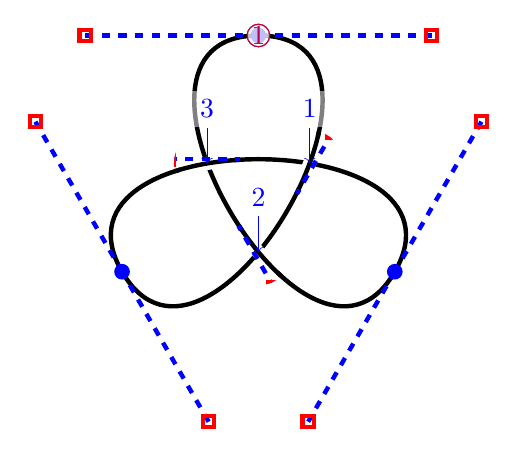
\begin{tikzpicture}
\begin{knot}[
  consider self intersections=true,
  draft mode=crossings, % comment this to hide the crossing numberings annotation
  flip crossing=2, % it's hard to see what the knot package names the crossings, 
  only when rendering/.style={
    show curve controls % comment this to hide controls annotations
  }
  ]
\strand (0,2) .. controls +(2.2,0) and +(120:-2.2) .. (210:2) .. controls +(120:2.2) and +(60:2.2) .. (-30:2) .. controls +(60:-2.2) and +(-2.2,0) .. (0,2);
\end{knot}
\end{tikzpicture}

\caption{The famous trefoil knot}
\end{figure}

From Wikipedia, the skein relation for the Conway polynomial is:

\begin{equation}
\nabla (L_{+})-\nabla (L_{-})=z\nabla (L_{0})
\end{equation}

I think that means the Conway polynomial of the trefoil knot is $z + 1$. 

\subsection*{A book you may enjoy flipping through: Differential Topology by Guilemin and Pollack \cite{guillemin2010differential}. Browse it and tell me what you think.}


It's somewhat interesting. It's terse and moves fast. I'm not sure I can do the exercises, but I'm not sure I can't do the exercises.

I feel like I recognize some stuff that it touches on.

The Euler Characteristic comes up a lot in Lakatos's Proofs and Refutations,
and deriving it for a manifold by counting self-intersections seems neato.

The ``mod 2'' counting stuff reminds me of something
that Jordan Ellenberg described Conway proving \cite{conway1983knots},
that given six points in general position in 3 space, there is always at least one way to join them to form a pair of linked triangles.

%    Bibliographies can be prepared with BibTeX using amsplain,
%    amsalpha, or (for "historical" overviews) natbib style.
\bibliographystyle{amsplain}
\bibliography{refs}

\end{document}

%%%%%%%%%%%%%%%%%%%%%%%%%%%%%%%%%%%%%%%%%%%%%%%%%%%%%%%%%%%%%%%%%%%%%%%%

%    Templates for common elements of a journal article; for additional
%    information, see the AMS-LaTeX instructions manual, instr-l.pdf,
%    included in the PROC author package, and the amsthm user's guide,
%    linked from http://www.ams.org/tex/amslatex.html .

%    Section headings
\section{}
\subsection{}

%    Ordinary theorem and proof
\begin{theorem}[Optional addition to theorem head]
% text of theorem
\end{theorem}

\begin{proof}[Optional replacement proof heading]
% text of proof
\end{proof}

%    Figure insertion; default placement is top; if the figure occupies
%    more than 75% of a page, the [p] option should be specified.
\begin{figure}
\includegraphics{filename}
\caption{text of caption}
\label{}
\end{figure}

%    Mathematical displays; for additional information, see the amsmath
%    user's guide, linked from http://www.ams.org/tex/amslatex.html .

% Numbered equation
\begin{equation}
\end{equation}

% Unnumbered equation
\begin{equation*}
\end{equation*}

% Aligned equations
\begin{align}
  &  \\
  &
\end{align}

%-----------------------------------------------------------------------
% End of proc-l-template.tex
%-----------------------------------------------------------------------